\section{Experiments}
\subsection{Linear experiment}
From the conclusions of aforementioned preliminary experiments, there are 6 usable PCs (PC2-PC7) and the original dataset has a dominating latent ability across all scenarios. To fit the ability model for each scenario, I created a Q-matrix which is a one-hot encoding matrix of the scenarios according to the ability dimensions. To fit the model, I used Multidimensional Item Response Theory (MIRT) \footnote{https://www.psychometrics.cam.ac.uk/system/files/documents/ multidimensional-item-response-theory.pdf} on the test set.

\[
p(y=1|\theta,a,d) = \sigma(a\cdot \theta - d)
\]

To verify if the dimensions are correlated with the accuracy of measured tasks, I conducted a report on the correlation of sub-scores with the original datasets ~\ref{PCA_subscore_corr}. The sub-scores are highly correlated with some original datasets, meaning they reflect similar skills or domains. When tested with the fit of thetas in 6 dimensions, the abilities displayed a weaker correlation with the original datasets. This may be explained by the strong general factor (g-factor) in the dataset. I performed an additional analysis taking into account that factor by appending an additional ability dimension which is shared by all datasets. This is called a Bi-factor model which separates a strong general factor and very specific ones. In any case, the correlation matrix showed significant noise. I also tested all of this approach with a larger question pool ($n\ge 40000$) but the model introduced even more noise.

\begin{figure}[!t]
    \centering
    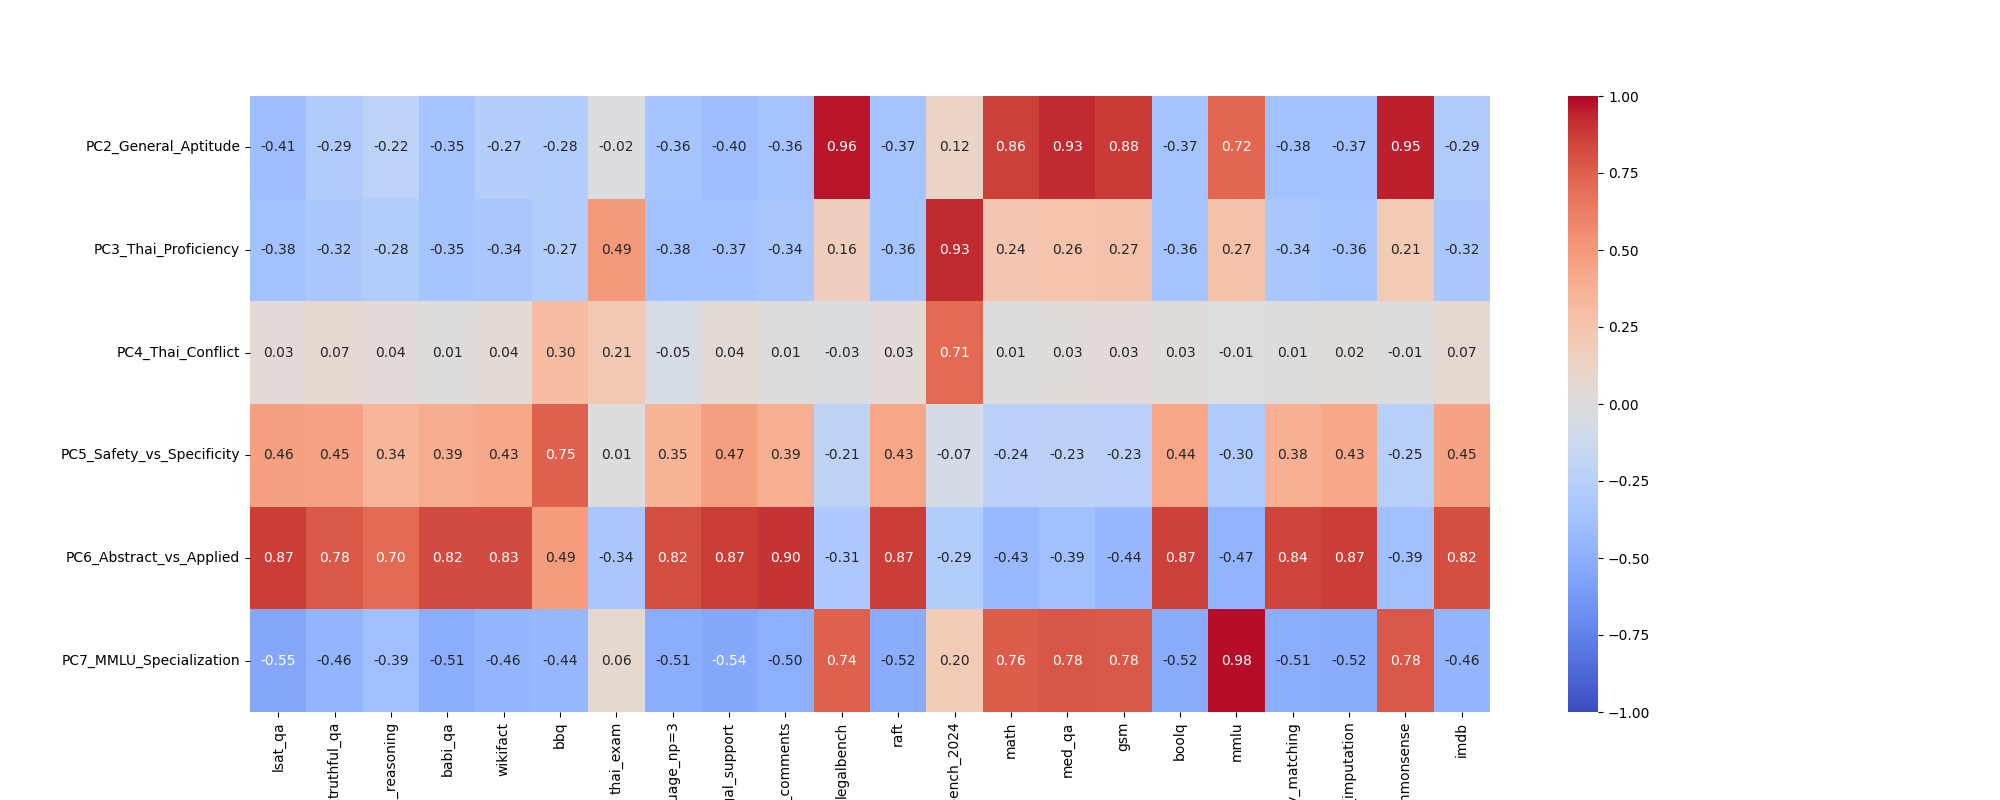
\includegraphics[width=\linewidth]{figures/PCA_subscore_corr.png}
    \caption{Correlation of Raw Sub-scores with original datasets.}
    \label{fig:PCA_subscore_corr}
\end{figure}

\begin{figure}[!t]
    \centering
    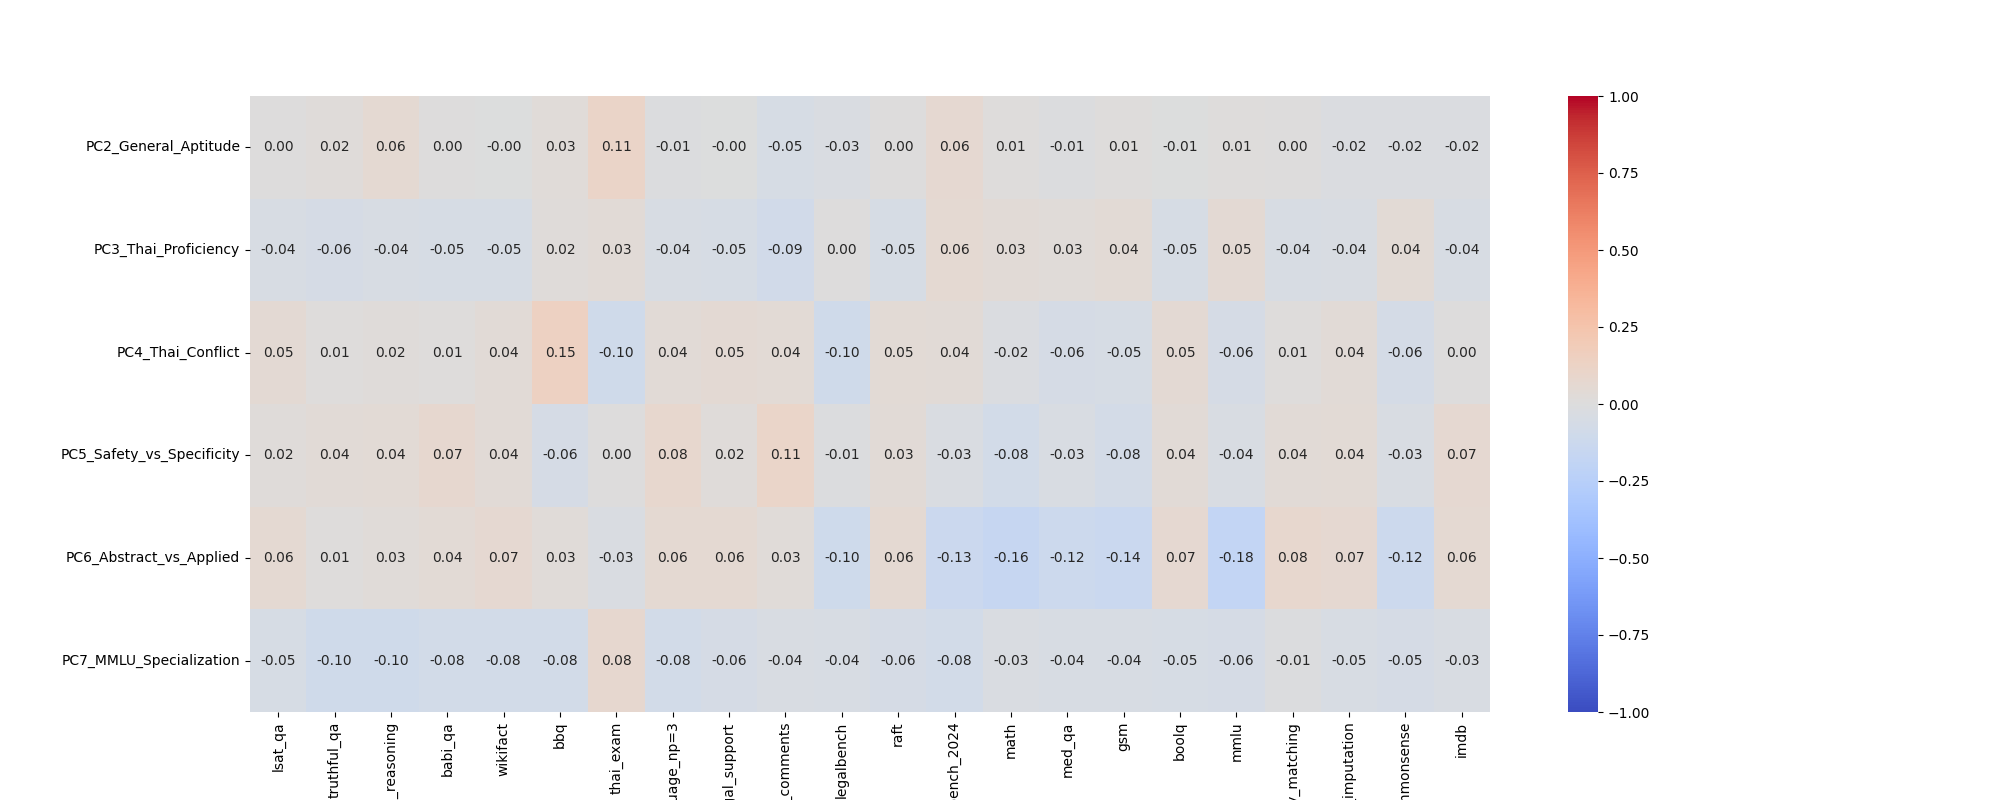
\includegraphics[width=\linewidth]{figures/PCA_testscore_corr.png}
    \caption{Correlation of $\gamma$ dimensions on MIRT 2-PL with the original dataset.}
    \label{fig:PCA_testscore_corr}
\end{figure}

\begin{figure}[!t]
    \centering
    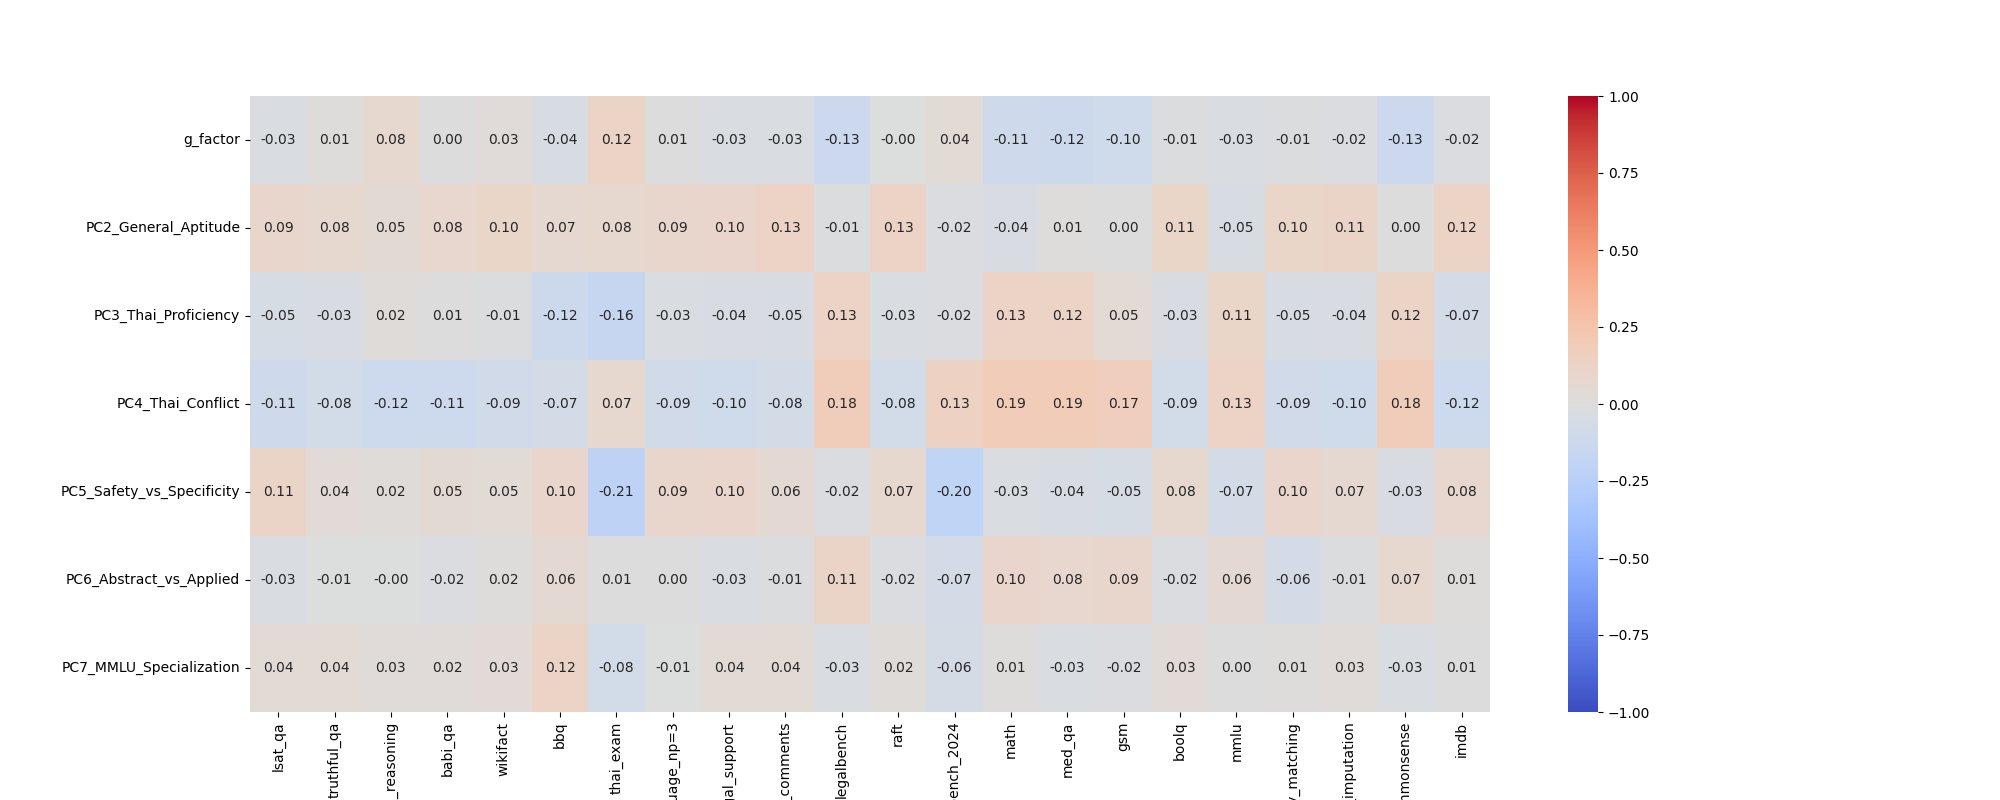
\includegraphics[width=\linewidth]{figures/PCA_g_testscore_corr.png}
    \caption{Correlation of $\gamma$ dimensions on MIRT 2-PL (Bi-factor model) with the original dataset.}
    \label{fig:PCA_g_testscore_corr}
\end{figure}

\subsection{Non-linear experiment}
Through the extensive survey, I have concluded that the regular, linear IRT model is insufficient to estimate the multidimensionality nature of the new $\gamma$. Another reasonable approach would be fitting the equation with a non-linear model, a Neural Network, which I find to have unanticipated success.

I reused the original IRT model to have a well-experimented reference. The new model is
\[
p(y=1|\theta, z)=\sigma(\mathcal{Q} \cdot \gamma - z)
\]
Where $\gamma=(\theta_1, \theta_2, \ldots, \theta_6)$ is the 6 dimensional ability encoding from PCA. In the neural network, $\gamma$ and $z$ are treated as learnable embeddings; whereas $\mathcal{Q}$ is treated as a non-trainable Q-matrix buffer. Putting this model through roughly half the response matrix ($n \approx 45000)$ and 5 epochs, I got improved results from the referenced experiment using the same measurement calculations.

%%%%%%%%%%%%%%% begin table   %%%%%%%%%%%%%%%%%%%%%%%%%%
\begin{table}[t]
\caption{Neural IRT Rasch model results}
\begin{center}
\label{table_ASME}
\begin{tabular}{l r r}
\cr \\ % put some space after the caption
\hline
Metric & Rasch Model & NeuralIRT \\
\hline
AUC Train & 0.840 & 0.970\\
AUC Test & 0.827 & 0.968 \\
Pearson Correlation & 0.999 & 0.999\\
Pearson Correlation & 0.993 & 0.999\\
\hline
\end{tabular}
\end{center}
\end{table}
%%%%%%%%%%%%%%%% end table %%%%%%%%%%%%%%%%%%% 

The result shows a clear correlation in some dimensions with the success rate of their corresponding upstream tasks. Furthermore, an analysis of the interactions between abilities signals an influence from some dimensions on another. This suggests one of two things: there are inherent, shared ability factor (g-factor) that makes some ability yield greater correlations than others (like logical reasoning would imply the improved performance on English and Maths tests), or if we consider the hypothesis of ability dimensions are strongly orthogonal, the definition of sub-ability needs to be refined. In any case, with the presence of absolute correlation, there's still a need for a more thorough and theoretically sound definition of PC or even an alternative approach to dimensionality reduction procedure to ensure the utmost reliability and validity of the test.

\begin{figure}[!t]
    \centering
    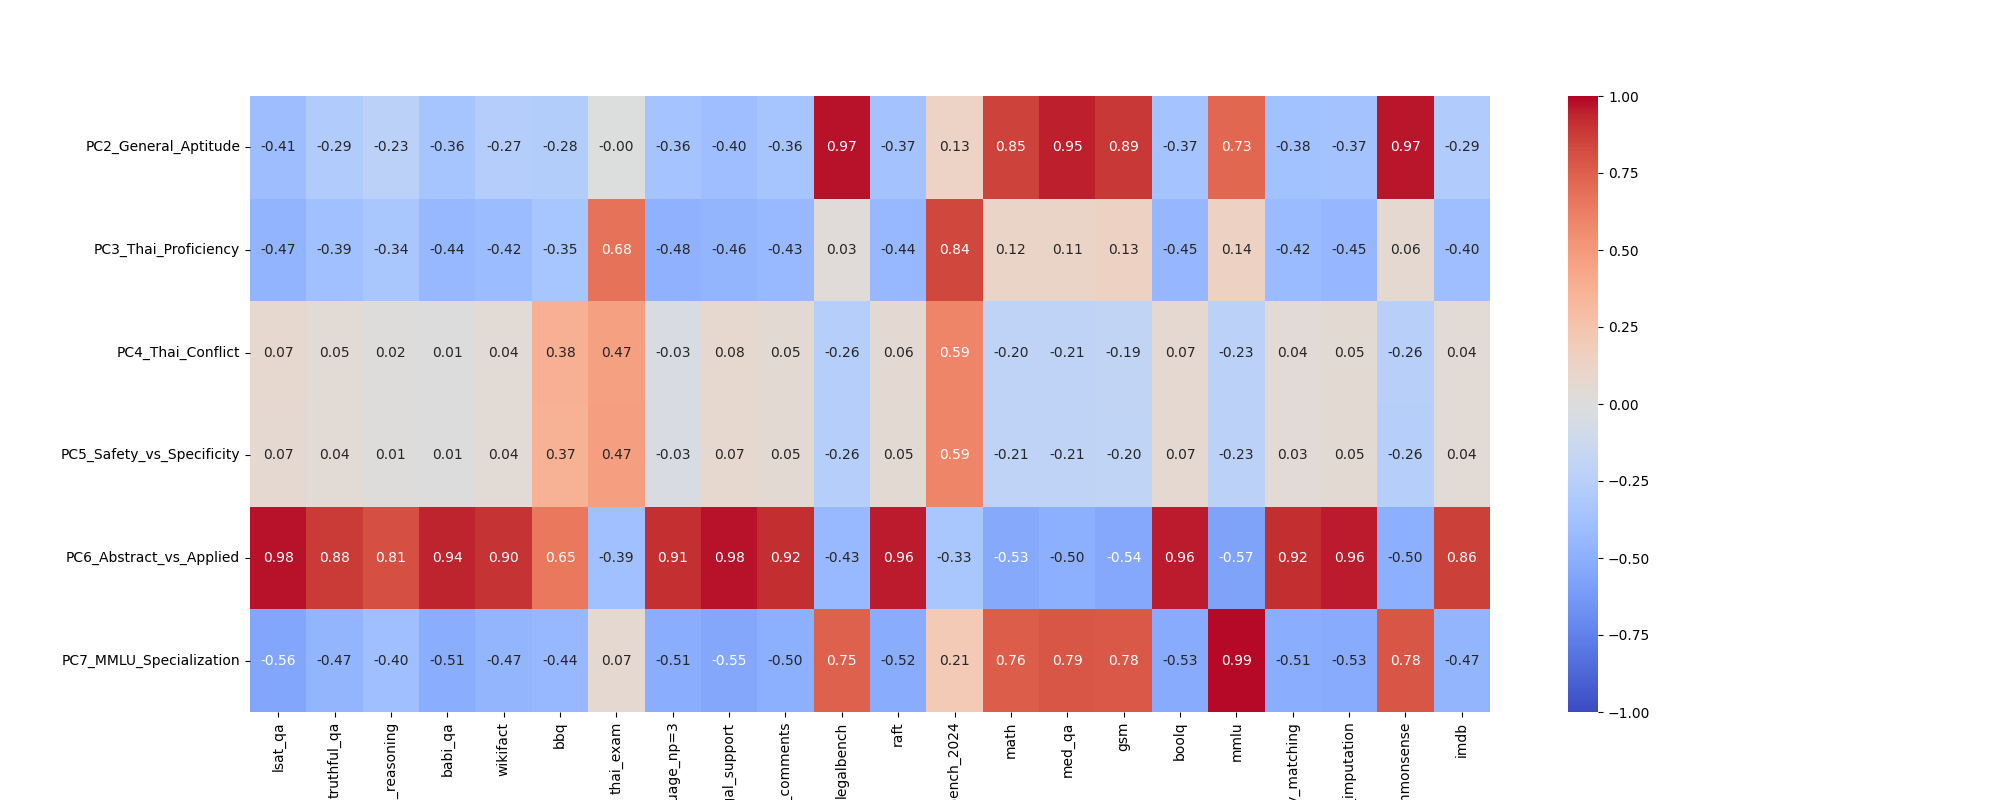
\includegraphics[width=\linewidth]{figures/external_validity_heatmap.png}
    \caption{Correlations of $\gamma$ dimensions on NeuralIRT to their upstream tasks.}
    \label{fig:external_validity_heatmap}
\end{figure}

\begin{figure}[!t]
    \centering
    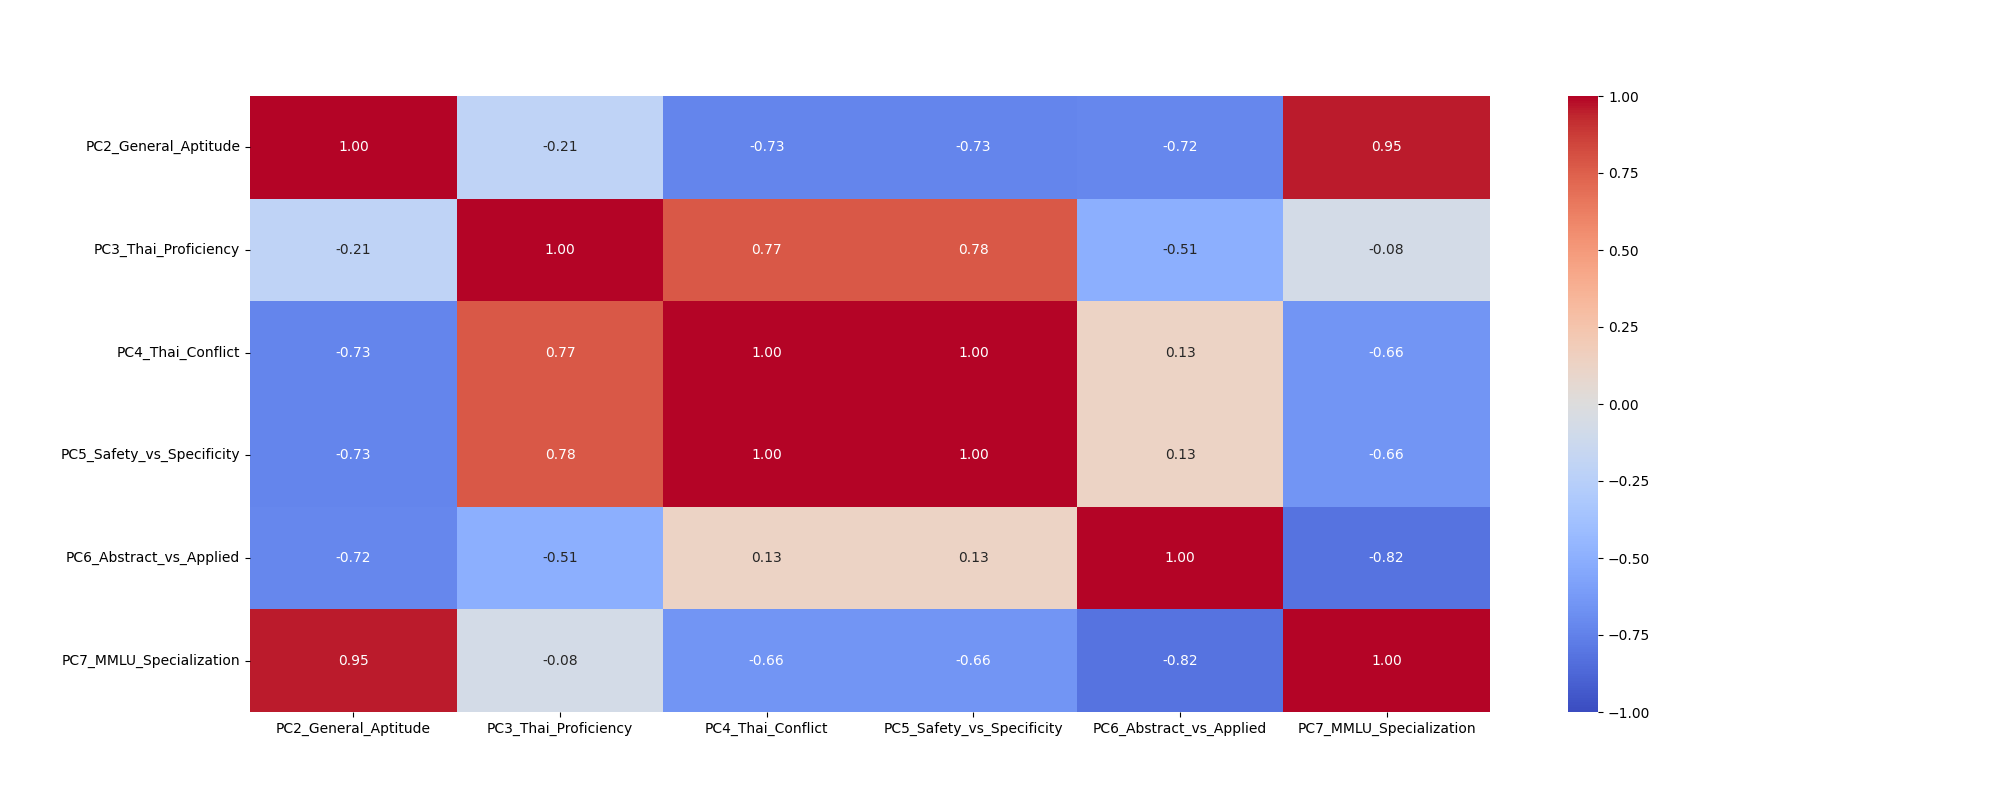
\includegraphics[width=\linewidth]{figures/theta_correlation.png}
    \caption{Correlation of $\gamma$ dimensions on NeuralIRT.}
    \label{fig:theta_correlation}
\end{figure}